%!TEX root = zukaFinalReport.tex
%!TEX encoding = UTF-8 Unicode
%==============================================================================

\section{Safe operating zone}
Vision technology has become a critical component for many robot applications, enabling robots to be deployed into new areas.  Over the years the technology has matured becoming very reliable, with higher performance and pricing has dropped dramatically.
Giving robots eyes enables them to perform increasing complex operations in ways that dramatically improve their performance. For example, robots guided by vision can locate parts to be picked up, determine where to apply a weld, inspect parts that have been assembled, determine where to place a part. The possibilities are endless.
The possibilities are not only limited to the industrial applications. For example, hand gestures can be used in teleoperation, navigation, or even to perform a surgery! [[[IEEE reference]]]. Computer vision libraries made it possible to detect human body and hence a safe operation zone can be provided. For more applications, you can have a look at this interesting IEEE article:
\url{http://spectrum.ieee.org/automaton/robotics/diy/top-10-robotic-kinect-hacks}

\section{State of the art}
One of the most important piece of information that a normal camera misses is the depth of the image. The depth is important in recognizing the real world in a proper way. Researchers had found many solutions for this problem like the stereo camera installations, or even including depth sensors with the RGB camera itself, like in the Kinect.
Kinect is a depth sensor which is able to return images like an ordinary camera, but instead of color, each pixel value represents the distance to the point. As such, the sensor can be seen as a range- or 3D-camera. For more technical details about Kinect, please refer to this website:

\url{https://ese.wustl.edu/ContentFiles/Research/UndergraduateResearch/CompletedProjects/WebPages/fl12/MattJohnson/kinect1.html}

Robotic grasping, object recognition, and human tracking became possible by interfacing Kinect camera to robots, especially robotic manipulators.

\section{What we have done}
We have used the Kinect and Robot Operating System (ROS) platform to implement two vision dependent systems on the KUKA robot:
\begin{itemize}
    \item Visual Servoing System, that makes the robot moves according to the tracked person’s hand position.
    \item Safe Operating Zone, where the robot slows down to 10% of its speed when a human is detected in the selected zone.
\end{itemize}

\section{Safe Operating Zone}
Human safety is the main concern which prevents performing some tasks requiring physical interaction between human and robot. Therefore, the safety concept was previously based on eliminating contact between human and robots.
Using vision system, we’ve made it possible for the robot to detect and recognize human body, and its distance to the fixed camera, hence a safe operating zone can be acquired by sending a signal to the robot to change its speed when a human is in the safety zone.
This is done by sending the RGB and depth data from the Kinect to the NiTE library, which is a middleware that provides body and skeleton detection, then reading this data by a ROS node to calculate the instantaneous distance of each human’s center of mass, and the signal is sent by another ROS node that listens to the stream of the least user distance.
\begin{figure}
    \centering
    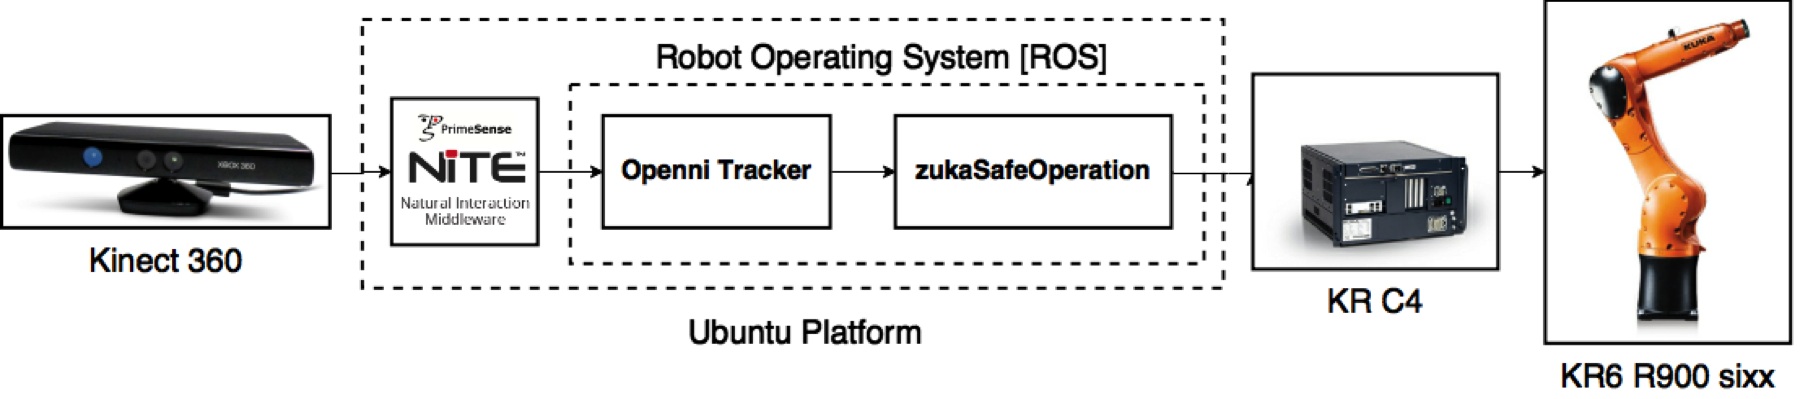
\includegraphics[width=\linewidth]{figures/kinectSaftyZone}
    \caption{Safe Operating Zone}
    \label{fig:kinectsaftyzone}
\end{figure}

\section{How to Use}
\begin{itemize}
\item Install kukavarproxy as explained before, and make sure that everything is ok
\item Install ROS, NiTE, and openni\_tracker as explained before
\item Launch the roscore, but don’t launch the openni\_tracker node
\item Copy the our modified openni\_tracker.cpp file to your catkin openni\_tracker package. Our node publish and extra topic called /closestUserDistance which gives the least detected distance of any tracked user without the need of standing in the psi calibration position
\item Copy the zukaSafeOperation package to your catkin workspace, and run catkin\_make to build the node. Don’t forget to change node mode to executable if it hasn’t.
\item Use: rosrun zukaSafeOperation zukaSafeOperation to launch the package
\item The package requires a proper internet connection through kukaproxvar, and changes the robot speed to 10\% of it’s speed when a user is detected within a range of 2 meters.
\end{itemize}

\paragraph{How to edit the detection data and the speed limits:}
In the source code you’ll find variables to define the range, and the limited speed. Change these variables to your desired ones

\paragraph{Where to download: }
\begin{itemize}
\item Edited openni\_tracker:  \url{https://github.com/mnourgwad/zuka/tree/master/codes/openni_tracker}
\item zukaSafeOperation:  \url{https://github.com/mnourgwad/zuka/tree/master/codes/zukaSafeOperation} 
\end{itemize}